%!TEX program = xelatex
% 完整编译: xelatex -> bibtex -> xelatex -> xelatex
\documentclass[lang=cn,11pt,a4paper,cite=numbers]{elegantpaper}
\usepackage{xfp}
\usepackage{tikz}

\title{Hyperbolic growth}
\author{Hui Zheng}
% \institute{}

% \version{0.09}
\date{\zhtoday}

% 本文档命令
\usepackage{array}
\newcommand{\ccr}[1]{\makecell{{\color{#1}\rule{1cm}{1cm}}}}

\begin{document}

\maketitle

\begin{abstract}
When a quantity grows towards a \href{https://en.wikipedia.org/wiki/Mathematical_singularity}{singularity} under a finite variation(a \href{https://en.wikipedia.org/wiki/Finite-time_singularity}{"finite-time singularity"}), it is said to undergo hyperbolic growth\cite{korotaev2006introduction}. More precisely, the \href{https://en.wikipedia.org/wiki/Reciprocal_function}{reciprocal function} $\frac{1}{x}$ has a \href{https://en.wikipedia.org/wiki/Hyperbola}{hyperbola} as a graph, and has a singularity at 0, meaning that the \href{https://en.wikipedia.org/wiki/Limit_of_a_function}{limit} as $x{\to}0$ is infinite: any similar graph is said to exhibit hyperbolic growth.
\begin{figure}[!htb]
  \centering
  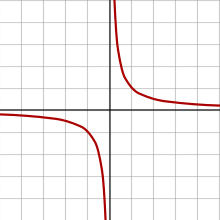
\includegraphics[width=0.4\textwidth]{figs/hyperbolic-growth.png}
  \caption{figs:hyperbolic-growth}
  \label{figs:hyperbolic-growth}
\end{figure}
\keywords{hyperbolic growth}
\end{abstract}

\section{Description}
  If the output of a function is \href{https://en.wikipedia.org/wiki/Inversely_proportional}{inversely proportional} to its input, or inversely proportional to the difference from a given value $x_{0}$, the function will exhibit hyperbolic growth, with a singularity at $x_{0}$.

  In the real world, hyperbolic growth is created by certain non-linear \href{https://en.wikipedia.org/wiki/Positive_feedback}{positive feedback} mechanisms\cite{markov2007phanerozoic}.

\subsection{Comparisons with other growth}
  Like \href{https://en.wikipedia.org/wiki/Exponential_growth}{exponential growth} and \href{https://en.wikipedia.org/wiki/Logistic_growth}{logistic growth}, hyperbolic growth is highly \href{https://en.wikipedia.org/wiki/Nonlinear_system}{nonlinear}, but differs in important respects. These functions can be confused, as exponential growth, hyperbolic growth, and the first half of logistic growth are \href{https://en.wikipedia.org/wiki/Convex_function}{convex functions}; however their \href{https://en.wikipedia.org/wiki/Asymptotic_behavior}{asymptotic behavior}(behavior as input gets large) differs dramatically.
\begin{itemize}
  \item logistic growth is constrained(has a finite limit, even as time goes to infinity),
  \item exponential growth grows to infinity as time goes to infinity (but is always finite for finite time),
  \item hyperbolic growth has a singularity in finite time (grows to infinity at a finite time).
\end{itemize}

\section{Mathematical example}
  The function
\begin{equation}
  x(t)=\frac{1}{t_{c}-t}
\end{equation}
exhibits hyperbolic growth with a singularity at time $t_{c}$: in the limit as $t{\to}t_{c}$, the function goes to infinity.

  More generally, the function
\begin{equation}
  x(t)=\frac{K}{t_{c}-t}
\end{equation}
exhibits hyperbolic growth, where $K$ is a scale factor.

  Note that this algebraic function can be regarded as analytical solution for the function's differential\cite{korotaev2006introduction}:
\begin{equation}
  \frac{dx}{dt}=\frac{K}{(t_{c}-t)^{2}}=\frac{x^{2}}{K}
\end{equation}

  This means that with hyperbolic growth the absolute growth rate of the variable $x$ in the moment $t$ is proportional to the square of the value of $x$ in the moment $t$. Respectively, the quadratic-hyperbolic function looks as follows:
\begin{equation}
  x(t)=\frac{K}{(t_{c}-t)^{2}}
\end{equation}

\section{See also}
\begin{itemize}
  \item \href{https://en.wikipedia.org/wiki/Exponential_growth}{Exponential growth}
  \item \href{https://en.wikipedia.org/wiki/Logistic_growth}{Logistic growth}
  \item \href{https://en.wikipedia.org/wiki/Mathematical_singularity}{Mathematical singularity}
\end{itemize}

\nocite{*}
\bibliography{ref/refs}

\end{document}
